% !TEX root = ../notes_template.tex
\chapter{Respiration}\label{chp:blood_oxygen}
Updated on \today
\minitoc
This chapter covers blood support of the extracellular fluid and cellular function by having the correct blood gases which is supported through Pulmonary (external) Respiration. Respiration is a microcirculation process that therefore requires concentration and pressure gradients as well as blood transport and circulation. Cellular (internal) Respiration occurs between the capillaries and muscle fibers and is supported by circulation. Pulmonary (external) Respiration is supported by Pulmonary Circulation (covered in this chapter). Just as Cellular Respiration includes a micro-circulatory exchange with muscle fibers, Pulmonary Respiration includes a micro-circulatory exchange with the the alveoli (air sacs) in the lung. Alveolar ventilation (covered in the next chapter) ensures that the alveoli maintain the required concentration (pressure) of both $CO_2$ and $O_2$ to support Pulmonary Respiration.

\vspace{5mm}

\textbf{Objectives include:}
\begin{enumerate}
    \item
    \item
    \item
    \item
    \item
\end{enumerate}

\section{Respiration Overview}
Muscle function requires energy in the form of ATP. Sustained regeneration of ATP in the mitochondria continuously produces $CO_2$ that must be removed from the muscle fiber, and requires $O_2$ which must be delivered to the muscle fiber. The microcirculation removes and provides what the muscle fibers need, including the removal of $CO_2$ and delivery of $O_2$ (Cellular Respiration). The microcirculation of the blood gases from and into muscle fibers requires a concentration gradient that requires a continuous circulation of blood to the muscle capillary network. Blood provides a transport mechanism for both $CO_2$ and $O_2$ (Blood Transport). The circulation of blood from the muscles through veins to the right side of the heart delivers all blood (venous return) to the pulmonary circulation. The pulmonary circulation delivers venous blood through pulmonary arteries to the interstitial space surrounding alveoli (air sacs) in the lungs (Pulmonary Circulation). Microcirculation (primarily gas diffusion) results in the equilibration of blood gases with the alveoli gases (Pulmonary Respiration). Pulmonary circulation then returns arterial blood through pulmonary veins to the left side of the heart for system wide distribution.


\section{Cellular Respiration}

The beginning of cellular respiration occurs inside the mitochondria with aerobic metabolism. It is aerobic metabolism that utilizes $O_2$ and produces $CO_2$ in sufficient quantities to require continuous exchange with the sarcoplasm, interstitial space, circulating blood and ultimately the environment (gas exchange). Cellular respiration establishes the need for what can be referred to as internal respiration, the gas exchange of $O_2$ and $CO_2$ between the intracellular and extracellular (both interstitial and vascular compartments. For simplicity we will use the terms cellular and internal respiration interchangeably.

\subsection{Partial Pressure Gradients \& Diffusion}

The fundamental concept for respiration is that partial pressure gradients of $O_2$ and $CO_2$ create pressure driven flow. For gases, pressure driven flow is typically called diffusion. There is a relationship between concentration and partial pressure. The higher the concentration of a particular molecule in a gas (as a fraction of all the molecules), the higher the partial pressure. Specifically, the partial pressure of a particular molecule in a gas is proportional to the number of particular molecules as a fraction of the total molecules of the gas multiplied by the total pressure of the gas. The partial pressure of $O_2$ being:

\begin{equation}
    PO_2 = FO_2 \times Total Pressure (mmHg)
    \label{PO2}
\end{equation}

Where $FO_2$ is the fraction of $O_2$ in the gas resulting in total pressure ($mmHg$). Air in the environment tends to have 21\% oxygen (as a fraction, 0.21). Air in the environment is inspired so is the fraction of inspired oxygen ($F_iO_2$). At sea level the total air pressure is 760 $mmHg$ (barometric pressure). Therefore, the $F_iO_2 = 0.21 \times 760 mmHg$, so $F_iO_2 = 159.5 mmHg$. 

\subsection{Partial Pressure Driven Diffusion}

Figure \ref{fig:ecf_respiration} is from Chapter \ref{chp:ecf_microcirculation}. Note that the gradients for $O_2$ and $CO_2$ are depicted as partial pressures ($PO_2$ and $PCO_2$). The partial pressure of each compartment is further noted with a subscript, with partial pressure of oxygen in the cell being $P_cO_2$ and in the tissue as $P_tO_2$. The gradient for $PO_2$ is from the arterial end of the capillary (partial pressure of arterial blood, $P_aO_2 \approx 100 mmHg$) into the tissue ($P_tO_2 \approx 40 mmHg$), and into the cell ($P_cO_2 \approx 20 mmHg$). Of these values the $P_cO_2$ is most variable and depends on the rate of utilization of $O_2$ in the mitochrondria (ETC). The partial pressure driven diffusion of cellular respiration relies on the continuous use of $O_2$ in the mitochondria; and the continuous use of $O_2$ in the mitochondria depends on the availability of $O_2$ diffusing in from the arterial blood in the capillary. If aerobic metabolism in a cell stopped then the $P_cO_2$ would quickly equilibrate with the $P_aO_2$ at 100 $mmHg$. If blood flow stopped (ischemia), or if there was a lower partial pressure of oxygen in the arterial blood ($P_aO_2 \leq 60 mmHg$) (hypoxemia) then diffusion of $O_2$ would be slower and the rate of aerobic metabolism (ETC in particular) would be limited (hypoxia).

\begin{figure}[!h]
    \centering
    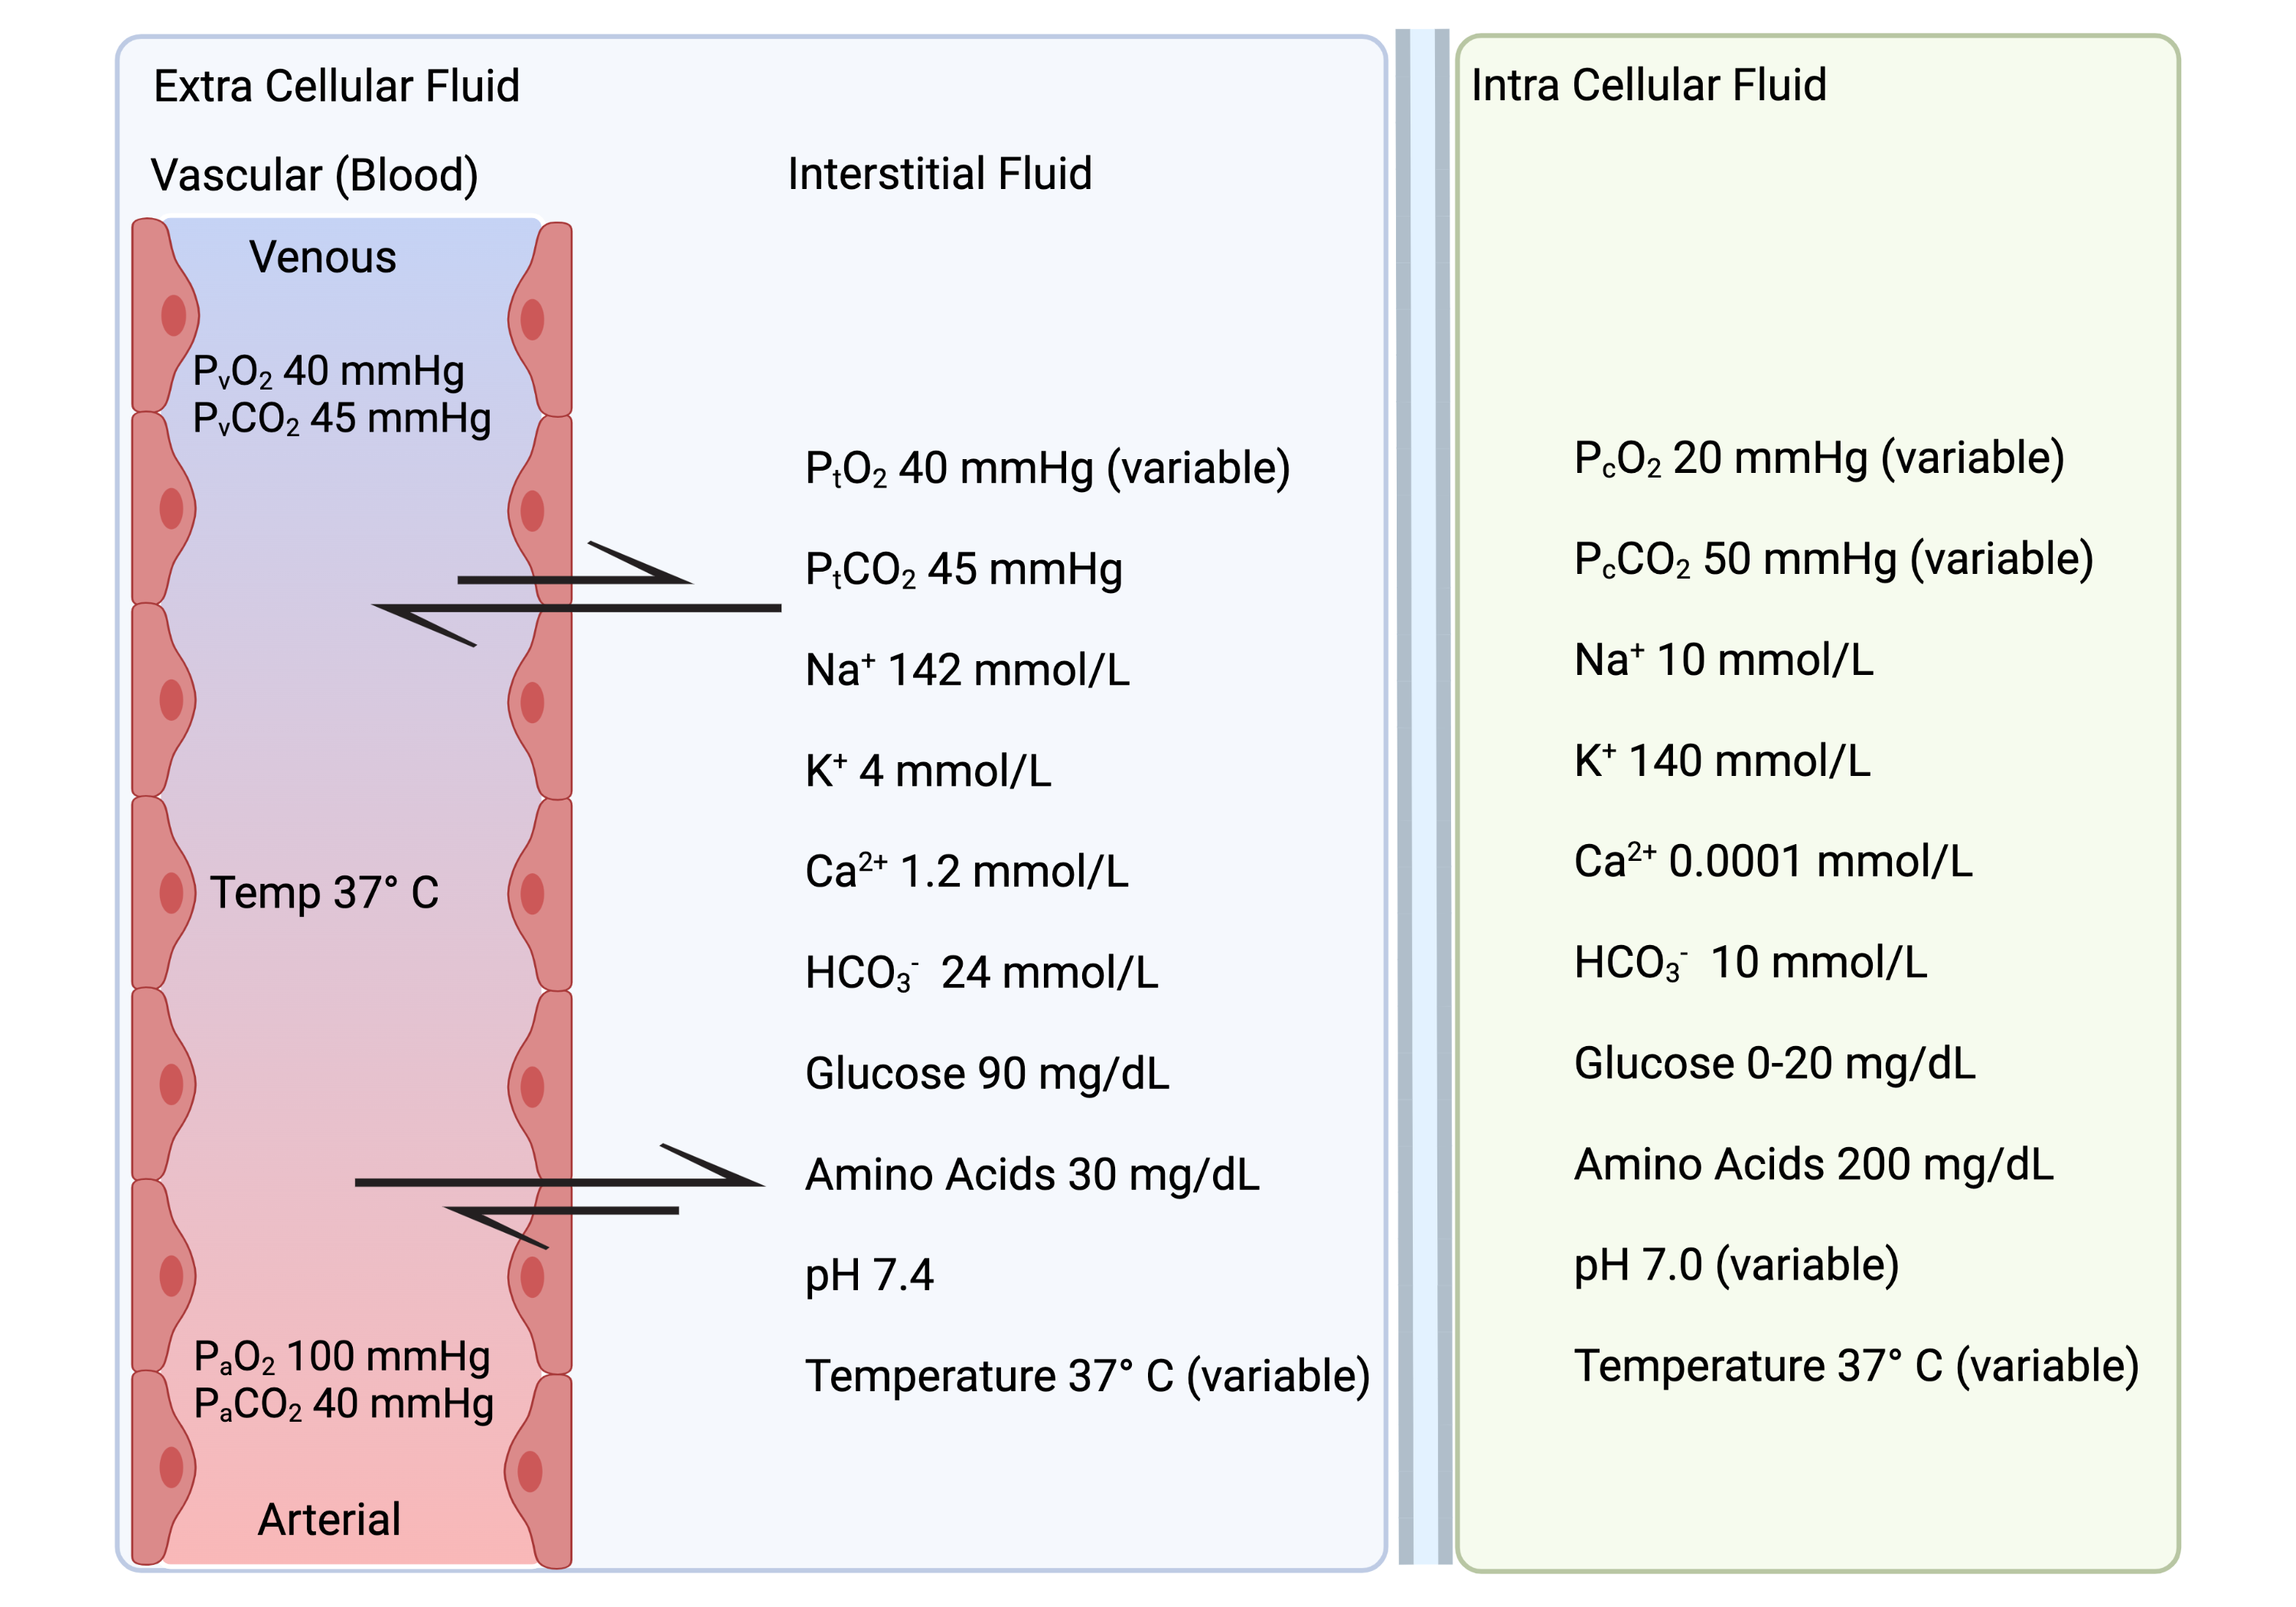
\includegraphics[width=1.0\linewidth]{./figure/ecf.png}
    \caption{Extra-cellular (Vascular \& Interstitial) and Intra-cellular Fluid \footnotesize{(Created with BioRender.com)}}
    \label{fig:ecf_respiration}
\end{figure}

The diffusion of $O_2$ into the tissue (interstitial space) reduces the partial pressure of $O_2$ in the blood. The $PO_2$ at the venous end of the capillary is the $P_vO_2$. An important concept is that the $P_vO_2$ from different areas of the body can be quite different. The regional $P_vO_2$ depends on the regional metabolism. While the $P_aO_2$ is the same throughout the arterial circulation, the $P_vO_2$ is different throughout the venous circulation, but continues to mix and become similar until the final mixing chambers of the right atrium and ventricles are reached. In other words, the $P_vO_2$ in the right ventricle represents a weighted mean from the entire body. And it is the $P_vO_2$ from the right ventricle that gets sent to the lungs, which means all of the alveoli receiving blood get blood with the same $PO_2$.

\paragraph{Carbon Dioxide}

Partial pressure driven diffusion of $CO_2$ follows the same reasoning as above but in the opposite direction. The $P_cCO_2$ is the highest partial pressure which drives diffusion of $CO_2$ out of the cell into the interstitial fluid. The $P_tCO_2$ is higher than the $Pa_CO_2$ in the arterial blood at the arterial end of the capillary, which drives $CO_2$ into the capillary. The $P_cCO_2$ is variable based on the rate of $CO_2$ produced during aerobic metabolism (TCA). The diffusion of $CO_2$ into the blood increases the $PCO_2$ in blood flowing through the capillary. At the venous end the $P_vCO_2$ equilibrates to whatever is in the tissue which is higher than the $P_aCO_2$. There tends be wider fluctuation in $P_aCO_2$ than in $P_aO_2$ due to the much lower atmospheric partial pressure of $CO_2$. For reasons that will be partially elucidated in this chapter and more fully explained in Chapter \ref{chp:alveolar_oxygen} on Ventilation, variation in ventilation (breathing rate and volume) can create large fluctuations in $P_aCO_2$ with relatively little change in $P_aO_2$. 







\section{Blood Transport}
\subsection{Blood Cells}

Blood cells

Blood - 0.6 plasma, 0.4 red blood cells 

Hematocrit is fraction that is RBC
Anemia (death < 0.10)

\subsection{Oxygen Transport - Red Blood Cells}


\section{Pulmonary Circulation}



\section{External (Alveolar) Respiration}



\paragraph{Atmospheric Limits}

The atmospheric $PO_2$ places a limit on how high the alveolar partial pressure ($P_AO_2$) can be and therefore how high the $P_aO_2$ can be. This upper limit means now matter how much someone breathes, there is an upper limit on diffusion of oxygen into the blood. That upper limit is reduced with lower atmospheric $PO_2$.


\subsection{Immunity - White Blood Cells}
% Role of lymph 
% Role of white blood cells
% Role of platelets

\subsection{Coagulation - Platelets}

\section{Oxygen}



\section{Carbon Dioxide}

\section{\textit{Connections:} Respiration Vital Signs}

\printbibliography[heading=subbibintoc]